\documentclass[master,otf]{gdutthesis}
\usepackage{mygdut}

\begin{document}
\graphicspath{{figures/}}

\frontmatter
%Environment fengmian
\begin{flushleft}
\hspace{8.5mm}
\includegraphics[height=2.19cm,width=2.21cm]{xiaohui.jpg} %校徽
\end{flushleft}
\begin{center} %居中环境 %图片

\includegraphics[height=2.96cm,width=10.56cm]{mingchen.jpg} %学校名字
\end{center}
\vspace{6.5mm}
\begin{center}
{\heiti \bfseries \yihao {本科毕业设计(论文)}}
\end{center}
\vspace{20mm}
\begin{center}
{\heiti \erhao \textbf{XXXXXXXXXXXXXXXXXXXXXXXXXXXXXX}}
\end{center}
\vspace{28mm}
\begin{center}
{\sanhao \heiti {学\hspace{2em}院\hspace{3mm}\dlmu{\textbf{物理光电工程学院}}}}\\\vspace{2.4mm}
{\sanhao \heiti {专\hspace{2em}业\hspace{3mm}\dlmu{\textbf{电子科学与技术}}}}\\\vspace{2.4mm}
{\sanhao \heiti {\hspace{4em}\hspace{3mm}\dlmu{\textbf{(微电子技术方向)}}}}\\\vspace{2.4mm}
{\sanhao \heiti {年级班别\hspace{3mm}\dlmu{\textbf{XXXXXXXXX}}}}\\\vspace{2.4mm}
{\sanhao \heiti {学\hspace{2em}号\hspace{3mm}\dlmu{\textbf{XXXXXXXX}}}}\\\vspace{2.4mm}
{\sanhao \heiti {学生姓名\hspace{3mm}\dlmu{\textbf{XX}}}}\\\vspace{2.4mm}
{\sanhao \heiti {指导教师\hspace{3mm}\dlmu{\textbf{XX}}}}
\end{center}
\vfill
\begin{center}
\makeatletter
\sanhao \heiti {\CJK@today}
\makeatother
\end{center}


\begin{cabstract}
LaTeX(/ˈlɑːtɛx/,常被读作/ˈlɑːtɛk/或/ˈleɪtɛk/),排版时通常使用\LaTeX{},是一种基于TeX的排版系统,由美国计算机科学家莱斯利·兰伯特在20世纪80年代初期开发,利用这种格式系统的处理,即使用户没有排版和程序设计的知识也可以充分发挥由TeX所提供的强大功能,不必一一亲自去设计或校对,能在几天,甚至几小时内生成很多具有书籍质量的印刷品。对于生成复杂表格和数学公式,这一点表现得尤为突出。因此它非常适用于生成高印刷质量的科技和数学、物理文档。这个系统同样适用于生成从简单的信件到完整书籍的所有其他种类的文档。

......
\end{cabstract}
\ckeywords{论文模板,\TeX{}~Live,\LaTeX{}}


\begin{eabstract}
\LaTeX{} is a document preparation system
for the \TeX{}   typesetting program. It offers
programmable desktop publishing features and
extensive facilities for automating most aspects
of typesetting and desktop publishing, including
numbering and cross-referencing, tables and figures,
page layout, bibliographies,   and much more.
\LaTeX{} was originally written in 1984 by Leslie
Lamport and has become the dominant method for
using \TeX; few people write in plain \TeX{} anymore.
The current version is  \LaTeXe.

......
\end{eabstract}
\ekeywords{Thesis Template, \TeX{} Live, \LaTeX{}}



% 生成目录
\tableofcontents

% 书写正文,可以根据需要增添章节。
\mainmatter
\chapter{模板编写}
《广东工业大学本科生毕业设计(论文)手册》\upcite{shouce}(下文简称《手册》)中对本科毕业论文构成、格式等作了详细的规定,编写一个符合这些规定的模板是本次设计的重要内容。本章将介绍论文模板编写的具体流程。

\section{宏包}
\TeX{} Live中有多种宏包供我们选择,我们用几个常用的宏包来构建我们的论文模板。见\tabref{package}。
\begin{table}[htbp]
\begin{center}
\caption{宏包名称及对应功能}
\label{tab:package}
\begin{tabularx}{\linewidth}{Z|Z|Z|Z|Z|Z} \toprule
宏包 & 功能 & 宏包 & 功能 & 宏包 & 功能 \\\cline{1-6}
geometry & 版面设置 & fancyhdr &  版式设计 & titlesec & 标题设置\\\cline{1-6}
titletoc & 目录设置 & graphicx & 插图 & subfig & 图片子标题\\\cline{1-6} 
float & 浮动体 & array & 数组 & booktabs & 线表格\\\cline{1-6}
tabularx & 可调列宽表格 & multirow & 跨行表格 & paralist & 列表\\\cline{1-6}
amsmath amssymb bm & 公式环境 & txfonts & 字体 & ntheorem & 定理\\\cline{1-6}
xeCJK & 中文支持 & indentfirst & 首行缩进 & natbib & 引用样式\\\cline{1-6}
hyperref & 超链接 & xcolor & 表格颜色 & listings & 代码\\\cline{1-6}
fancyvrb & 抄录环境 & algorithm & 算法环境 & & \\\bottomrule
\end{tabularx}
\end{center}
\end{table}

模板使用命令\verb|\RequirePackage|加载,用法

{\centering {\verb|\RequirePackage[参数1,参数2,参数3......]{宏包}|}\\}

如:

{\centering {\verb|\RequirePackage[center,pagestyles]{titlesec}|}\\}

\section{基本设置}
\subsection{字体}
\label{sec:font}
\TeX{}的字体设置比较麻烦,因此要用到XeCJK宏包。我们定义了几种文字,如\tabref{font},以便于我们编写使用。同时也支持Adobe公司的字体库。假如运行在Linux下,默认的系统字体不适合书写文档\upcite{linuxfont},建议使用Adobe公司的字体库。
\begin{table}[htbp]
\begin{center}
\caption{字体设定}
\label{tab:font}
\begin{tabularx}{\linewidth}{ZZZZ} \toprule
字体 & 命令 & Windows 7 & Adobe\\\cline{1-4}
Times New Roman & \multicolumn{3}{c}{无需设定,\LaTeX{}自带} \\
宋体 & \verb|\song| & SimSun & Adobe Song Std \\
黑体 & \verb|\hei| & SimHei & Adobe Heiti Std \\\bottomrule
\end{tabularx}
\end{center}
\end{table}

用\verb|\setCJKfamilyfont|设置字体的自定义名称,用法

{\centering {\verb|\setCJKfamilyfont{自定名称}{字体名称}|}\\}

如:

{\centering {\verb|\setCJKfamilyfont{kai}{Adobe Kaiti Std}|}\\}

\subsection{字号}
\label{sec:fontsize}
\LaTeX{}中的字体大小一般都用pt做单位\upcite{point},跟我们平时熟悉的在Word中的四号、五号字格式不同,所以可以根据对应关系定义新指令,用来在后面的编写中方便地改变字号,这里仅提供论文要用到的字体大小,其他大小不予给出,如\tabref{fontsize}。
\begin{table}[hbpt]
\begin{center}
\caption{字号设置}
\label{tab:fontsize}
\begin{tabularx}{\linewidth}{ZZZZZZZZ}\toprule
字号 & 大小(pt)& 字号 & 大小(pt)& 字号 & 大小(pt)& 字号 & 大小(pt)\\\cline{1-8}
二号 & 22pt & 小二 & 18pt & 三号 & 16pt & 四号 & 14pt \\
小四 & 12pt & 五号 & 10.5pt & 小五 & 9pt & & \\\bottomrule
\end{tabularx}
\end{center}
\end{table}

用\verb|\newcommand{}|设置字号的自定义名称,用法

{\centering {\verb|\newcommand{命令}{\fontsize{大小}{行距}\selectfont}|}\\}

如:

{\centering {\verb|\newcommand{erhao}{\fontsize{22pt}{\baselineskip}\selectfont}|}\\}

\subsection{中文元素}
默认的页面元素的英文名,诸如Contents 为目录,Abstract 为摘要等,我们首先将他们一一中文化,需要中文化的元素如\tabref{element}
\begin{table}[htbp]
\begin{center}
\caption{元素}
\label{tab:element}
\begin{tabularx}{\linewidth}{ZZZZZZ}\toprule
元素 & 中文 & 英文 & 元素 & 中文 & 英文 \\\midrule
目录 & content & 目 录 & 致谢 & 致~谢 & Acknowledgements \\
公式 & equation & 公式 & 参考文献 & 参~考~文~献 & References \\
图片 & figure & 图 & 表格 & 表 & table\\
附录 & Appendix & 附录 & 年月 & 2013年6月 & 2013.6 \\\bottomrule
\end{tabularx}
\end{center}
\end{table}

\section{版式}
学校规定,学位论文文稿用A4 纸( 210mm×297mm )标准大小的白纸双面打印,论文装订后尺寸为标准A4 纸的尺寸,一律在左侧装订,要求装订、剪切整齐,便于使用和保存。

本模板设置上边距30mm,下边距25mm ,左边距30mm和右边距20mm ,页脚顶部到版心距离10mm,到页面底边距离15mm,由于此宏包的页脚高度不计入页边距里,所以,实际的页边距为25mm=10mm+15mm直到比对正确为止,设定如下:

{\centering {\textbackslash geometry\{top=28mm,bottom=15mm,left=30mm,right=20mm,nohead,footskip=10mm\}}\\}

\section{页脚}
《手册》中的页脚格式为绪论至附录有页脚,模板中设置一个无页脚的空页面和一个有页脚的页面。绪论之前的页面都是用无页脚模式。
\begin{lstlisting}
\fancypagestyle{plain}{\renewcommand{\headrulewidth}{0pt}\fancyhf{}} %`无页脚`
\fancypagestyle{mainpage}{
\fancyhf{}
\fancyfoot[ER,OR]{\thepage} %`页脚始终在右边`
} 
\end{lstlisting}

\section{编写格式}
当页面设置好之后,就是在论文的不同部分分别调用,一般来说论文类的书籍分为三个matter ,为前言区(前置部分),正文区(主体),后文区(附录),在《手册》中要求,绪论至附录要求有页码,且封面,摘要及目录不计入页码。

首先看前置部分,主要包括封面,摘要,目录等,实现为:
\begin{lstlisting}
\renewcommand\frontmatter{%
    \if@openright\cleardoublepage\else\clearpage\fi
    \@mainmatterfalse
	\fancyhf{}
    \pagestyle{plain}
}
\end{lstlisting}
其中\verb|\@mainmatterfalse|为停止章节计数器,即前面的章节均假如正文的章节计算。

之后为文章的正文区,采用阿拉伯数字编页码:
\begin{lstlisting}
\renewcommand\mainmatter{%
    \if@openright\cleardoublepage\else\clearpage\fi
    \@mainmattertrue
    \pagenumbering{arabic}
    \sihao
    \def\@tabular{\wuhao[1]\old@tabular} % 之后表格字体使用5号
    \pagestyle{mainpage}
  }
\end{lstlisting}
其中\verb|\normalsize|为正文的字体、字号、间距等设置,\ref{sec:normalsize}~条将会提到。

附录属于后文区,具体设置见\ref{sec:appendix}~条。

\section{摘要}
模板为摘要做了一个专门的环境,符合《手册》上的规定。
\begin{lstlisting}[language=TeX]
\newenvironment{cabstract}{%
  \titleformat*{\chapter}{\xiaosan \heiti \filcenter \bfseries}
  \chapter*{\cabstractname}
  \xiaosi
  \@afterheading} %`保留章节标题下的首行段落的空白`
{\par\vspace{1em}\par}
\end{lstlisting}
中文摘要设为不参与排序的节,所以使用了\textbackslash chapter*\{\textbackslash cabstractname\},中间上方的星号意为不参与排序。由于不需求页码,所以在Thesis.tex文件加载摘要前加入\textbackslash frontmatter。

\section{目录}
目录用\verb|\tableofcontents|即可以很方便地自动生成。按照《手册》要求,自动生成的目录还不符合格式要求,用titletoc宏包来制定目录的样式。用法:

{\centering {\verb|\titlecontents{标题层次}[左间距]{整体格式}|
\verb|{标题序号}{标题 内容}{指引线和页码}[下间距]|}\\}

如:

{\centering {\verb|\titlecontents{chapter}[0pt]{\vspace{6bp} \heiti \xiaosi[1]}|
\verb|{\thecontentslabel\quad}{}{\titlerule*{.}\contentspage}|}\\}

\section{正文部分}
\subsection{正文标题}
《手册》规定了正文各级标题的格式,可调用titlesec宏包来设置。用法,

{\centering{\verb|\titleformat{标题层次}{整体格式}{标题 序号}{序号与内容间距}{标题内容}|}\\}

如:

{\centering {\verb|\titleformat{\chapter}{\filcenter \heiti \bfseries \sanhao}{\thechapter}{1em}{}|}\\}

目录的层次深度为条,即第三级,所以模板设置为\textbackslash setcounter\{secnumdepth\}\{3\}。
\subsection{正文字体}
\label{sec:normalsize}
首先确定正文中使用的字体,文档要求正文字体为小四,行距为1.5倍,中文字体为宋体,英文为Times New Roman。

由于大部分人习惯用Word里的行距,所以经过微调后,设置\textbackslash baselinestretch为1.25倍。

\subsection{正文段落}
文档设定为首行缩进2个字符,这一个命令需要在文档开始时自动执行:

{\centering {\verb|\setlength{\parindent}{2.5em}|}\\}
2.5em值得是2.5个字符量,由2em经过实际微调而得到。

定义段落间距,段前间距以及段后间距都为0。

{\centering {\verb|\setlength{\parskip}{0bp \@plus .5bp \@minus .5bp}|}\\}

\section{浮动对象}
浮动对象针对的目标是图片表格,标题为五号字体,图片标题在下,表格标题在上。具体设置:
\begin{lstlisting}[language=TeX]
\setlength{\floatsep}{12bp \@plus 2bp \@minus 1bp}
\setlength{\intextsep}{12bp \@plus 2bp \@minus 1bp}
\setlength{\textfloatsep}{12bp \@plus 2bp \@minus 1bp}
\setlength{\@fptop}{0bp \@plus1.0fil}
\setlength{\@fpsep}{8bp \@plus2.0fil}
\setlength{\@fpbot}{0bp \@plus1.0fil}
\renewcommand{\textfraction}{0.15}
\renewcommand{\topfraction}{0.85}
\renewcommand{\bottomfraction}{0.65}
\renewcommand{\floatpagefraction}{0.80}
\let\old@tabular\@tabular
\DeclareCaptionLabelFormat{tabularlabel}{{\wuhao \heiti #1~\rmfamily #2}}
\DeclareCaptionLabelFormat{figurelabel}{{\wuhao \song #1~\rmfamily #2}}
\DeclareCaptionLabelSeparator{floatsong}{\hspace{1em}}
\DeclareCaptionFont{tabularcap}{\wuhao \bfseries \heiti }
\DeclareCaptionFont{figurecap}{\wuhao }
\captionsetup[table]{position=top,belowskip=-0.2em,aboveskip=0.1em,labelformat=tabularlabel,labelsep=floatsong,font=tabularcap}
\captionsetup[figure]{position=bottom,belowskip=-0.2em,aboveskip=0.1em,labelformat=figurelabel,labelsep=floatsong,font=figurecap}
\captionsetup[subfloat]{justification=centering}
\renewcommand{\thesubfigure}{(\alph{subfigure})}
\renewcommand{\thesubtable}{(\alph{subtable})}
\end{lstlisting}

\section{封面}
\label{sec:cover}
封面的组成是两个不浮动的图片(校徽、校名称),加上\textbackslash vspace\{\}间距控制和几行文字组成。其中的图片大小皆符合《手册》给出的大小。而间距控制根据《手册》以及实际生成的封面进行对比微调。直接给出代码:

\begin{lstlisting}[language=TeX]
\begin{flushleft}
\hspace{8.5mm}
\includegraphics[height=2.19cm,width=2.21cm]{xiaohui.jpg} %`校徽`
\end{flushleft}
\begin{center} 

\includegraphics[height=2.96cm,width=10.56cm]{mingchen.jpg} %`学校名字`
\end{center}
\vspace{6.5mm}
\begin{center}
{\heiti \yihao {`本科毕业设计(论文)`}}
\end{center}
\vspace{20mm}
\begin{center}
{\heiti \erhao \textbf{`XXXXXXXXXXXXXXXXXXXXXX`}}
\end{center}
\vspace{25mm}
\begin{center}
{\sanhao \heiti {`学`\hspace{2em}`院`\hspace{3mm}\dlmu{\textbf{`物理光电工程学院`}}}}\\\vspace{2.5mm}
{\sanhao \heiti {`专`\hspace{2em}`业`\hspace{3mm}\dlmu{\textbf{`电子科学与技术`}}}}\\\vspace{2.5mm}
{\sanhao \heiti {`年级班别`\hspace{3mm}\dlmu{\textbf{`XXXXXX`}}}}\\\vspace{2.5mm}
{\sanhao \heiti {`学`\hspace{2em}`号`\hspace{3mm}\dlmu{\textbf{XXXXXXXX}}}}\\\vspace{2.5mm}
{\sanhao \heiti {`学生姓名`\hspace{3mm}\dlmu{\textbf{`XX`}}}}\\\vspace{2.5mm}
{\sanhao \heiti {`指导教师`\hspace{3mm}\dlmu{\textbf{`XX`}}}}
\end{center}
\vspace{20mm}
\begin{center}
\makeatletter
\sanhao \heiti {\CJK@today}
\makeatother
\end{center}
\end{lstlisting}

假如需要修改封面,直接在Cover.tex修改即可。

\section{参考文献}
根据《手册》上的规定,模板为摘要做了一个专门的环境。代码如下:

\begin{lstlisting}[language=TeX]
\renewenvironment{thebibliography}[1]{%
  \thispagestyle{emptypage}
  \chapter*{\bibname}%
  \addcontentsline{toc}{chapter}{`参考文献`}
  \list{\@biblabel{\@arabic\c@enumiv}}%
  {\renewcommand{\makelabel}[1]{##1\hfill}
    \setlength{\labelsep}{1ex}
    \setlength{\itemindent}{0pt}
    \setlength{\leftmargin}{\labelwidth+\labelsep}
    \addtolength{\itemsep}{-1em}
    \usecounter{enumiv}%
    \let\p@enumiv\@empty
    \renewcommand\theenumiv{\@arabic\c@enumiv}}%
  \sloppy\frenchspacing
  \clubpenalty4000%
  \@clubpenalty \clubpenalty
  \widowpenalty4000%
  \interlinepenalty4000%
  \sfcode‘\.\@m
}
\end{lstlisting}

根据《手册》中的具体打印实例,在目录中,“参考文献”各个字中间无须加入空格。但在章节标题时需要加入空格。所以使用\textbackslash addcontentsline\{toc\}\{chapter\}\{参考文献\},以区分章节标题及目录标题。

\section{致谢}
致谢的要求如“参考文献”。在目录中,各个字中间无须加入空格,但在章节标题时需要加入空格。所以,另外为致谢做了一个环境。代码如下:

\begin{lstlisting}[language=TeX]
\newenvironment{ack}{%
  \thispagestyle{emptypage}
  \chapter*{\ackname}%
  \addcontentsline{toc}{chapter}{`致谢`}%
  \xiaos
  \@mainmatterture
  \@afterheading
}
{\par\vspace{2em}\par}
\end{lstlisting}

\section{附录}
\label{sec:appendix}
最后是附录部分,由于他的章节标题与正文中不一样(不是第几章,而是附录A),同时《手册》中的实际打印效果是“目录中的附录条目不带附录标题内容”同时“附录实际页面中标题既带有附录标签同时带有附录标题内容”。这个设定与\LaTeX{}自动生成的有比较大的出入。所以从新设定了三个计数器以及一个附录环境。

代码如下:

\begin{lstlisting}[language=TeX]
\newcounter{appx}[chapter]
\renewcommand{\theappx}{\Alph{appx}}
\newcommand{\appx}[1]{\refstepcounter{appx}%
\begin{center}
\heiti \bfseries \sanhao{\par{`附录`}\textbf{\theappx}\quad#1}
\end{center}
\vspace{0.8em}}

\newcounter{appxtab}[appx]
\renewcommand{\theappxtab}{\theappx\arabic{appxtab}}
\newcommand{\appxtab}{\refstepcounter{appxtab}\centering \heiti \bfseries {\par{`表`\hspace{0.2em}}\theappxtab}\quad}

\newcounter{appxfig}[appx]
\renewcommand{\theappxfig}{\theappx\arabic{appxfig}}
\newcommand{\appxfig}{\refstepcounter{appxfig}\centering \song{\par{`图`\hspace{0.2em}}\theappxfig\quad}}

\newcommand{\appxtoc}[1]{\appx{#1}\par\addcontentsline{toc}{chapter}{`附录`\theappx}}

\newenvironment{appxchp}{%
\@afterheading%
\clearpage}{}
\end{lstlisting}

其中包含了附录章节、附录表格、附录图片计数器。\textbackslash appxtoc被定义为附录章的标题,同时为目录添加一条附录目录。《手册》中不要求附录中有节条等多级标题,所以没加入此功能。

\chapter{使用此模板}

\section{自动生成}
何为自动生成?

此模板的编写完全遵守《广东工业大学本科生毕业设计(论文)》的要求。你只需要用上以下会提到的一些注意要点,同时学习简单使用\TeX{}Maker或其他\TeX{}编辑器,编写好\TeX{}文件,加载本模板,并且运行批处理命令或自动运行脚本,成功编译后,你就能得到一份格式正确的论文。所有你所需要努力的就是写一个好的论文内容。免除格式的烦恼。关于编译,详细请看\ref{sec:compile}节。

\section{封面}
直接修改Cover.tex即可。详情看\ref{sec:cover}节。

\section{摘要}
模板已经设定好了摘要的环境,直接填入摘要文字,及关键字文字即可。
\begin{lstlisting}
\begin{cabstract}%`中文摘要`
\end{cabstract}
\ckeywords{`中文关键词`}
\begin{eabstract} %abstract
\end{cabstract}
\ekeywords{keywords}
\end{lstlisting}

\section{目录}
目录环境已经在模板内定义,直接使用\verb|\tableofcontents|命令即可。

\section{正文}
正文的文字书写环境已经模板内清楚定义,直接书写即可。换行的时候要注意,在\TeX{}源文件中,换行需要用到命令\verb|\\|、\verb|\par|或换两行(即使用两次回车键)。

\subsection{标题}
正文标题按级填写,不建议超过三级。
\begin{lstlisting}[language=TeX]
\chapter{`章标题`}
\section{`节标题`}
\subsection{`条标题`}
\end{lstlisting}

\subsection{字号及字符}
字符的设定及使用,见\ref{sec:fontsize}节;字号的设定及使用,见\ref{sec:font}节。

\subsection{特殊字符}
一些特殊符号需要用\TeX{}命令来表示,如\tabref{char}。\TeX{}Maker有直接生成数字符号的功能,方便大家使用。
\begin{table}[htbp]
\begin{center}
\caption{特殊字符输入}
\label{tab:char}
\begin{tabularx}{\linewidth}{Z|Z|Z|Z|Z|Z|Z|Z|Z|Z} \toprule
输入 & \verb|\#| & \verb|\$| & \verb|\%| & \verb|\&| & \verb|\{| & \verb|\}| & \verb|\_| & \verb|\^{}| & \verb|\~{}| \\\cline{1-10}
显示 & \# &	\$ & \% & \& & \{ & \} & \_	& \^{} & \~{} \\\cline{1-10}
输入 & \multicolumn{2}{Z|}{\verb|\textless|} & \multicolumn{2}{Z|}{\verb|\textgreater|} & \multicolumn{2}{Z|}{\verb|\textbar|} & \multicolumn{3}{Z}{\verb|\textbackslash|} \\\cline{1-10}
显示 & \multicolumn{2}{Z|}{\textless} & \multicolumn{2}{Z|}{\textgreater} & \multicolumn{2}{Z|}{\textbar} & \multicolumn{3}{Z}{\textbackslash} \\\bottomrule
\end{tabularx}
\end{center}
\end{table}

\section{插入表格}
此节介绍表格的画法。从简单的三线表,到复杂的内嵌表格。当然,你也直接可以用\TeX{}Maker画出你所需要的表格。根据《手册》中的规定,不介绍跨页表格的画法,需要跨页表格,可以通过分表格的方法。

\subsection{三线表}
表格的画法可以直接表现为线条的组合。如\tabref{tabexample1},仿制自《手册》24页的表3.3。

\begin{table}[htbp]
\begin{center}
%\caption{压降损失计算结果}
\Ucaption{压降损失计算结果}{Pa}
\label{tab:tabexample1}
\begin{tabularx}{\linewidth}{ZZZ}\toprule
换热器 & 热边压降损失 & 冷边压降损失\\\midrule
初级 & 2974.37 & 2931.52\\
次级 & 2924.65 & 3789.76\\\bottomrule
\end{tabularx}
\end{center}
\end{table}

代码如下:

\begin{lstlisting}[language=TeX]
\begin{table}[htbp]
\begin{center}
\caption{压降损失计算结果}\raisebox{0.75em}[-1.2em]{\hspace*{0.5\linewidth}\heiti \bfseries Pa}
\label{tab:tabexample1}
\begin{tabularx}{\linewidth}{ZZZ}\toprule
`换热器` & `热边压降损失` & `冷边压降损失`\\\midrule
`初级` & 2974.37 & 2931.52\\
`次级` & 2924.65 & 3789.76\\\bottomrule
\end{tabularx}
\end{center}
\end{table}
\end{lstlisting}

假如制作简单的表格可以直接用此模板。在table的浮动环境下,设定一个居中的环境,在居中环境里面添加标题\textbackslash caption。加入引用标签\textbackslash label,这样就可以随时在正文中使用\textbackslash tabref命令引用相关表格。接下来就是画表,使用四周(上下左右)居中的环境Z,表格宽度为版心宽度\textbackslash linewidth。\textbackslash toprule为顶边的线,midrule为中间的线,bottomrule为底边线。

需要注意的是,由于\tabref{tabexample1}比较特殊,在标题后面有一个标记压强单位Pa,所以用了\textbackslash raisebox命令建立了一个向上移动0.75个字符,深度(即字体间距)为-1.2个字符的上升盒子来装“Pa”。这个并非必须,这个功能类似于Word里面的文本框功能,当你想放置一些无序的内容时,可以使用它。

\subsection{复杂表格}
复杂表格\tabref{tabexample2},仿制自《手册》24页的表2.1。

\begin{table}[htbp]
\begin{center}
\caption{方法——干扰抑制结果}
\label{tab:tabexample2}
\begin{tabularx}{\linewidth}{Z|Z|Z|Z|Z} \toprule
干扰类型 & 目标信号 & 阵元数 & 干扰采样指数 & SINR(dB) \\\cline{1-5}
\multirow{4}*{第一类干扰} & \multirow{2}*{信号1} & 8 & -- & 30.58 \\\cline{3-5} 
& & 4 & -- & 21.16 \\\cline{2-5} 
& \multirow{2}*{信号4} & 8 & -- & 38.28 \\\cline{3-5} 
& & 4 & -- & 19.41 \\\hline
\multirow{3}*{第二类干扰} & \multirow{3}*{信号4} & \multirow{2}*{8} & 30 & 4.69 \\\cline{4-5} 
& & & 19 & 4.83 \\\cline{3-5} 
& & 4 & 30 & -4.42 \\\bottomrule
\end{tabularx}
\end{center}
\end{table}

代码如下:

\begin{lstlisting}[language=TeX]
\begin{table}[htbp]
\begin{center}
\caption{`方法——干扰抑制结果`}
\label{tab:tabexample2}
\begin{tabularx}{\linewidth}{Z|Z|Z|Z|Z} \toprule
`干扰类型` & `目标信号` & `阵元数` & `干扰采样指数` & SINR(dB) \\\cline{1-5}
\multirow{4}*{`第一类干扰`} & \multirow{2}*{`信号1`} & 8 & -- & 30.58 \\\cline{3-5} 
& & 4 & -- & 21.16 \\\cline{2-5} 
& \multirow{2}*{`信号4`} & 8 & -- & 38.28 \\\cline{3-5} 
& & 4 & -- & 19.41 \\\hline
\multirow{3}*{`第二类干扰`} & \multirow{3}*{`信号4`} & \multirow{2}*{8} & 30 & 4.69 \\\cline{4-5} 
& & & 19 & 4.83 \\\cline{3-5} 
& & 4 & 30 & -4.42 \\\bottomrule
\end{tabularx}
\end{center}
\end{table}
\end{lstlisting}

表格假如需要全局的竖线,可以直接在Z环境后加上竖线如\{Z\textbar Z\textbar Z\}。由于有一些格需要跨行合并,所以需要\textbackslash multirow命令,multirow\{4\}*\{第一类干扰\}代表者跨4行,×表示数据自然高度,\{\}里为内容。\textbackslash cline命令可以设置划线的列数,例如\textbackslash cline{3-5}为从第三列画到第5列。\textbackslash hline可以画出与表格宽度相等的线,类似于\textbackslash midrule。

要注意,被合并行是从上往下数,即第一行合并了下面的二、三、四行,所以二、三、四行的第一个空个的内容皆为空。

介绍另外一种复杂表格,需要用到列合并。复杂表格\tabref{tabexample3},仿制自《手册》24页的表3.1(摘其中几行作为示例)。

\begin{table}[htbp]
\begin{center}
\caption{各分组lgB$_{i}$值}
\label{tab:tabexample3}
\begin{tabularx}{\linewidth}{ZZZZZ} \toprule
\multirow{2}*{序号} & \multicolumn{2}{|c|}{\textit{T}=1500K} & \multicolumn{2}{c}{\textit{T}=2000K} \\\cline{2-5}
 & \multicolumn{1}{|Z}{组分} & \multicolumn{1}{|Z|}{lgB$_{i}$} & 组分 & \multicolumn{1}{c}{lgB$_{i}$} \\\midrule
1 & O$_{2}$$^{+}$ & 5.26 & HO$_{2}$ & 6.43 \\
6 & OH & 3.29 & OH & 5.91 \\
10 & H$_{2}$O$_{2}$ & 1.62 & CO$_{2}$$^{+}$ & 3.76 \\
12 & HCO$^{*}$ & -0.47 & HCO$^{*}$ & 0.24 \\\bottomrule
\multicolumn{5}{l}{\xiaowu 注:“+”表示重要部分,“*”表示冗余组分。} \\
\end{tabularx}
\end{center}
\end{table}

代码如下:

\begin{lstlisting}[language=TeX]
\begin{table}[htbp]
\begin{center}
\caption{`各分组lgB$_{i}$值`}
\label{tab:tabexample3}
\begin{tabularx}{\linewidth}{ZZZZZ} \cline{1-5}
\multirow{2}*{`序号`} & \multicolumn{2}{|c|}{\textit{T}=1500K} & \multicolumn{2}{c}{\textit{T}=2000K} \\\cline{2-5}
 & \multicolumn{1}{|Z}{`组分`} & \multicolumn{1}{|Z|}{lgB$_{i}$} & `组分` & \multicolumn{1}{c}{lgB$_{i}$} \\\cline{1-5}
1 & O$_{2}$$^{+}$ & 5.26 & HO$_{2}$ & 6.43 \\
6 & OH & 3.29 & OH & 5.91 \\
10 & H$_{2}$O$_{2}$ & 1.62 & CO$_{2}$$^{+}$ & 3.76 \\
12 & HCO^{*} & -0.47 & HCO$^{*}$ & 0.24 \\\cline{1-5}
\multicolumn{5}{l}{\xiaowu `注:“+”表示重要部分,“*”表示冗余组分。`} \\
\end{tabularx}
\end{center}
\end{table}
\end{lstlisting}

\textbackslash multicolumn命令是列合并。\textbackslash multicolumn\{2\}\{\textbar c\textbar\}\{\textbackslash textit\{T\}=1500K\}表达的意思是合并2列表格,合并后的表格内容居中并且两边生成竖边框,内容为斜体的T=1500K。\textbackslash multicolumn命令运作方式与\textbackslash multicolumn有所不同,如第一行,由于\textbackslash multicolumn命令的作用,该行仅有三个空需要填入内容。假如需要行列合并的话,可以使用\textbackslash multicolumn\{行数\}\{对齐\}\{\textbackslash multirow\{列数\}*\{内容\}\}

关于脚注,由于《手册》中要求脚注前要加上注,\textbackslash footnote命令无法达到效果,所以建议用\textbackslash multicolumn命令生成一个左对齐的无边框单行表格,然后直接输入相关文字即可。

另外,\verb|\^{}|为上标,\verb|\_{}|为下标。可以直接用\TeX{}Maker生成。

\subsection{子表格}
子表格经常用于表格之间的比对。如,\tabref{parallel1}、\tabref{parallel2}

\begin{table}[htbp]
\noindent\begin{minipage}{0.45\textwidth}
\centering
\caption{第一个并排子表格}
\label{tab:parallel1}
\begin{tabularx}{0.45\textwidth}{Z|Z}
\toprule
111 & 222 \\\midrule
222 & 333 \\\bottomrule
\end{tabularx}
\end{minipage}
\begin{minipage}{0.45\textwidth}
\centering
\caption{第二个并排子表格}
\label{tab:parallel2}
\begin{tabularx}{0.45\textwidth}{Z|Z}
\toprule
111 & 222 \\\midrule
222 & 333 \\\bottomrule
\end{tabularx}
\end{minipage}
\end{table}

代码如下:

\begin{lstlisting}[language=TeX]
\begin{table}[htbp]
\noindent\begin{minipage}{0.45\linewidth}
\centering
\caption{`第一个并排子表格`}
\label{tab:parallel1}
\begin{tabularx}{0.45\linewidth}{Z|Z}\toprule
111 & 222 \\\midrule
222 & 333 \\\bottomrule
\end{tabularx}
\end{minipage}
\begin{minipage}{0.45\linewidth}
\centering
\caption{`第二个并排子表格`}
\label{tab:parallel2}
\begin{tabularx}{0.45\linewidth}{Z|Z}\toprule
111 & 222 \\\midrule
222 & 333 \\\bottomrule
\end{tabularx}
\end{minipage}
\end{table}
\end{lstlisting}

用小页环境minipage,把table环境分割成为两小块,每块为版心宽的0.45倍。

除了使用小页环境之外,我们也可以用子表格环境。如\tabref{subtable}。

\begin{table}[htbp]
\centering
\caption{并排子表格}
\label{tab:subtable}
\subfloat[第一个子表格]{
\begin{tabularx}{0.4\linewidth}{Z|Z}\toprule
111 & 222 \\\midrule
222 & 333 \\\bottomrule
\end{tabularx}}\hspace{0.15\linewidth}
\subfloat[第二个子表格]{
\begin{tabularx}{0.4\linewidth}{Z|Z}\toprule
111 & 222 \\\midrule
222 & 333 \\\bottomrule
\end{tabularx}}
\end{table}

代码如下:

\begin{lstlisting}[language=TeX]
\begin{table}[htbp]
\centering
\caption{`并排子表格`}
\label{tab:subtable}
\subfloat[`第一个子表格`]{
\begin{tabularx}{0.4\linewidth}{Z|Z}\toprule
111 & 222 \\\midrule
222 & 333 \\\bottomrule
\end{tabularx}}\hspace{0.15\linewidth}
\subfloat[`第二个子表格`]{
\begin{tabularx}{0.4\linewidth}{Z|Z}\toprule
111 & 222 \\\midrule
222 & 333 \\\bottomrule
\end{tabularx}}
\end{table}
\end{lstlisting}

由于《手册》中并未明确表明可以使用子表格,仅供大家参考。

\section{插图}
本章简单介绍一些在《手册》下适用的插图方法,假如需要了解更多,建议读一下《\LaTeXe 插图指南》\upcite{graphics}。

\subsection{单个图形}
\figref{figexample1}仿照《手册》的22页的图2.3。

\begin{figure}[htbp]
\begin{center}
{\rotatebox{90}{\hspace{13.5mm} \xiaowu 所有用户的平均误差比特率}}{\hspace{15mm}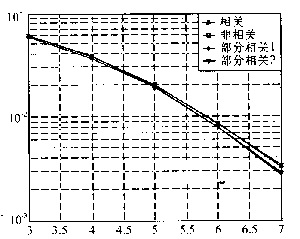
\includegraphics[height=65mm]{1.jpg}}{\hspace*{20mm}}
\end{center}
\vspace{-1.5em}
\hspace{-4em} {\xiaowu[0.75] 信噪比/dB}\\
{\centering {\xiaowu[0.75] \noindent 注:此图中的曲线对应关系与图2.1相同.}\\}
\caption{部分相干调解与相干和非相干调解平均误码性能的比较}
\label{fig:figexample1}
\end{figure}

代码如下:

\begin{lstlisting}[language=TeX]
\begin{figure}[htbp]
\begin{center}
{\rotatebox{90}{\hspace{13.5mm} \xiaowu `所有用户的平均误差比特率`}}{\hspace{15mm}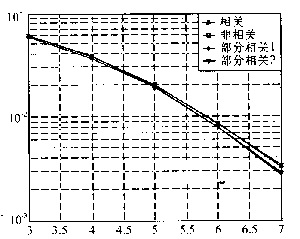
\includegraphics[height=65mm]{1.jpg}}{\hspace*{20mm}}
\end{center}
\vspace{-1.5em}
\hspace{-4em} {\xiaowu[0.75] `信噪比/dB`}\\
{\centering {\xiaowu[0.75] \noindent `注:此图中的曲线对应关系与图2.1相同.`}\\}
\caption{`部分相干调解与相干和非相干调解平均误码性能的比较`}
\label{fig:figexample1}
\end{figure}
\end{lstlisting}

主体部分是\textbackslash includegraphics[高度]\{图片\}。

另外,为了达到原图的效果,使用了\textbackslash rotatebox,旋转盒子的命令,把文字旋转90度至于图片左边。又通过用\textbackslash hspace\{\},水平间距命令及\textbackslash vspace\{\},垂直间距命令,把“信噪比/dB”放置于对齐于图片的左下角。同时使用\textbackslash centering命令把注解居中于图标题上方。以达到图2.3的效果。

字号的中括号内容表示行距设定。\LaTeX{}的行距设定在换字号大小的时候才会生效。为了使表格的注解能够比较紧凑,用0.75倍的行距比较适宜。

下\figref{figexample2}仿制《手册》22页的图3.1。

\begin{figure}[htbp]
\begin{center}
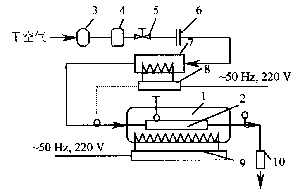
\includegraphics[height=50mm]{2.png}\\
{{\xiaowu[0.75]{1-太阳模拟器;2-单管及31个PCM容器;3-气泵;\\
4-干燥过滤器;5-手动调节阀;6-孔板流量计;\\
7-空气预热器;8,9-调功器;10-空气换热器。\\}}}
\end{center}
\caption{单管换热系统流程图}
\label{fig:figexample2}
\end{figure}

代码如下:

\begin{lstlisting}[language=TeX]
\begin{figure}[htbp]
\begin{center}
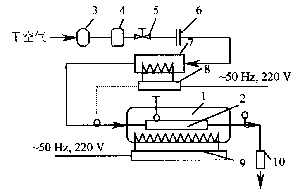
\includegraphics[height=50mm]{2.png}\\
{{\xiaowu[0.75]{`1-太阳模拟器;2-单管及31个PCM容器;3-气泵;`\\
`4-干燥过滤器;5-手动调节阀;6-孔板流量计;`\\
`7-空气预热器;8,9-调功器;10-空气换热器。`\\}}}
\end{center}
\caption{单管换热系统流程图}
\label{fig:figexample2}
\end{figure}
\end{lstlisting}

相较\figref{figexample1},\figref{figexample2}显得简单得多,我们的插图一般以这种为主。

\subsection{多个图形}
多个图形的编排与多个表格的编排基本相同,可以用小页minipage分割,或者使用subfigure子图片环境。

\figref{figexample3}展示的是《手册》23页的图2.5。

\begin{figure}[htbp]
\centering
\subfloat[分布符合1/f规律图]{%
\label{fig:subfig1}
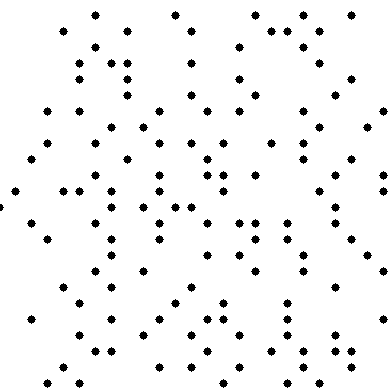
\includegraphics[height=40.8mm]{3.png}}\hspace{4em}%
\subfloat[大小与色彩符合1/f规律图]{%
\label{fig:subfig2}
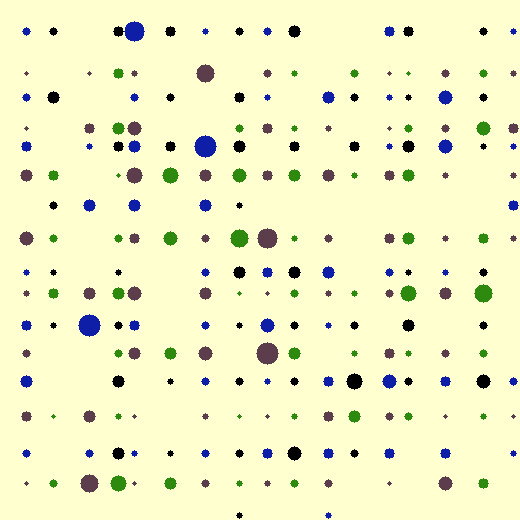
\includegraphics[height=38.4mm]{4.png}}\hspace{4em}
\subfloat[间距、大小与色彩均符合1/f规律图]{%
\label{fig:subfig3}
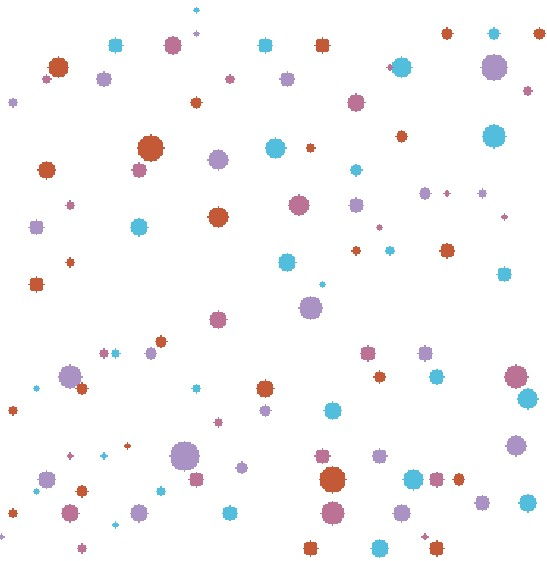
\includegraphics[height=41.7mm]{5.jpg}}
\caption{图案例}
\label{fig:figexample3}
\end{figure}

代码如下:

\begin{lstlisting}[language=TeX]
\begin{figure}[htbp]
\centering
\subfloat[`分布符合1/f规律图`]{%
\label{fig:subfig1}
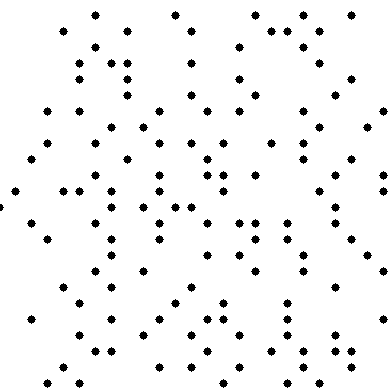
\includegraphics[height=40.8mm]{3.png}}\hspace{4em}%
\subfloat[`大小与色彩符合1/f规律图`]{%
\label{fig:subfig2}
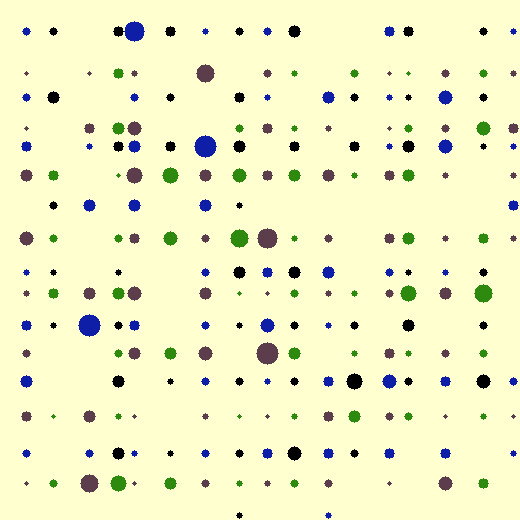
\includegraphics[height=38.4mm]{4.png}}\hspace{4em}
\subfloat[`间距、大小与色彩均符合1/f规律图`]{%
\label{fig:subfig3}
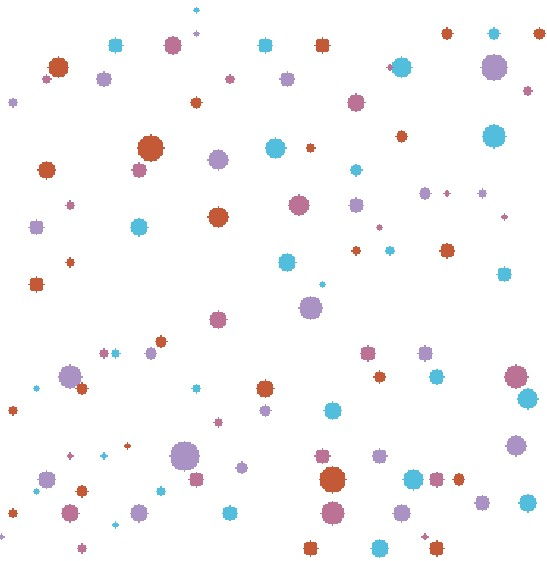
\includegraphics[height=41.7mm]{5.jpg}}
\caption{`图案例`}
\label{fig:figexample3}
\end{figure}
\end{lstlisting}

需要注意的是,图与图之间的间距,需要用水平间距命令进行调整。

\section{公式定理}
\TeX{}处理公式的能力非常强大,建议读取amsmath宏包的说明文档\upcite{amsmath}。下面举几个简单的例子,皆在公式环境equation中生成,对付不同的公式已经够了。其中的数学符号,可以在Web Equation网页中手写生成。

\begin{figure}[htbp]
\begin{center}
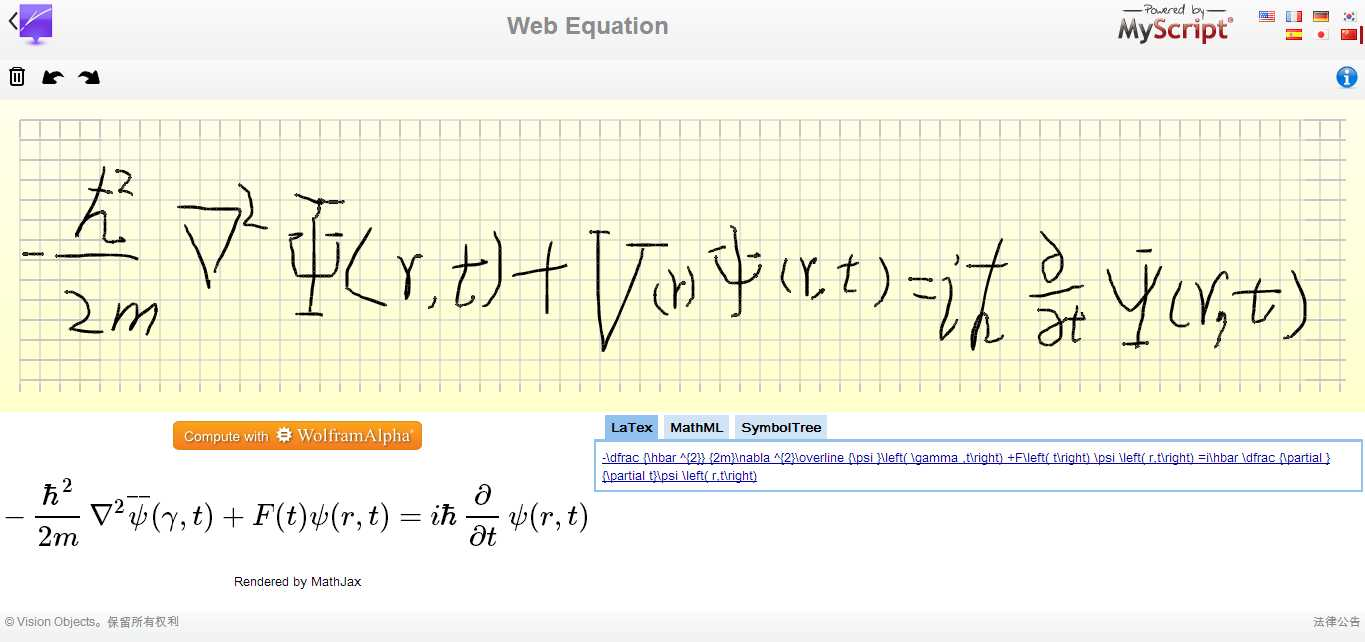
\includegraphics[width=0.9\linewidth]{wq.png}
\end{center}
\caption{用Web Equation生成\TeX{}公式代码}
\end{figure}

\subsection{单个公式}

\newcommand{\envert}[1]{\left\lvert#1\right\rvert} 
\begin{equation}\label{detK2}
\det\mathbf{K}(t=1,t_1,\dots,t_n)=\sum_{I\in\mathbf{n}}(-1)^{\envert{I}}
\prod_{i\in I}t_i\prod_{j\in I}(D_j+\lambda_jt_j)\det\mathbf{A}
^{(\lambda)}(\overline{I}|\overline{I})=0.
\end{equation} 

\begin{multline}%\tag{[b]} % 这个出现在索引中的
\int_a^b\biggl\{\int_a^b[f(x)^2g(y)^2+f(y)^2g(x)^2]
 -2f(x)g(x)f(y)g(y)\,dx\biggr\}\,dy \\
 =\int_a^b\biggl\{g(y)^2\int_a^bf^2+f(y)^2
  \int_a^b g^2-2f(y)g(y)\int_a^b fg\biggr\}\,dy
\end{multline}

\subsection{多列公式}

\begin{equation} 
\overrightarrow {p}_{i}\left( u\right) =\sum _{j=0}^{k}\overrightarrow {V}_{i}\Lambda _{i}\left( k;\overrightarrow {\beta }_{1},\ldots \overrightarrow {\beta }_{n};u\right)
\end{equation}

\begin{equation} 
\dfrac {\left| A\left( s\right) \right| ^{2}} {\left| A\left( O\right) \right| ^{2}}=\dfrac {\rho _{1}\rho _{2}} {\left( s+p_{1}\right) \left( s+\rho _{2}\right) }
\end{equation}

\section{代码高亮}
有些时候我们需要在论文中引入一段代码。
在模板中,统一使用\textbackslash listings宏包,并且设置了基本的内容格式。由于Lstlisting宏包对中文支持不太完善,可以设置中文逃逸,\textbackslash lstset\{escapeinside=\`{}\`{}\},用键盘数字符号键“1”左边的“倒引号”“\`{}”作为逃逸标记。但请注意,在Verilog语言中,左引号为特殊符号。

C语言示例:

\begin{lstlisting}[language=C]
#include <stdio.h>
main()
{printf("Hello World!\n"); %"`你好,世界`"
}
\end{lstlisting}

\section{参考文献}
参考文献可以用thebibliography环境生成,代码如下:

\begin{lstlisting}[language=TeX]
\begin{thebibliography}{}
\bibitem[`序号`]{`引用`} `文献信息`
\bibitem[1]{b1} Wikipedia. Linux[EB/OL]. http://zh.wikipedia.org/wiki/Linux,2013-5-20/2013-5-26. 
\end{thebibliography}
\end{lstlisting}

其中[]中填入文献前标号,缺省为数字排列,\{\}中为引用标签,例如\{r1\}则可在其他地方用指令\verb|\cite{r1}|引用标签上标可以使用\textbackslash textsuperscript命令,用法与\textbackslash cite一样。

\section{致谢}
致谢可以直接使用ack环境。直接输入文字即可。

\section{附录}
使用appxchp环境,在环境里使用\textbackslash appxtoc\{标题内容\}生成符合《手册》要求的附录。同时如需要生成图或表格的标题,使用\textbackslash appxfig(图) 和\textbackslash appxtab(表) 命令。引用标题的方法与正文相同。其他的操作与正文一样。

\section{编译}
\label{sec:compile}
好的,恭喜你,你终于写完了\TeX{}原文档了。是时候开始编译了。但在这之前,你还需要以下步骤:

1、创建一个空文件夹,名称如:gdutthesis

2、把thesis.tex、gdutthesis.cls、mygdut.sty、makepdf.bat、makefile三个文件放到你新建的文件夹里。

3、在这个新文件夹下建立两个新的空文件夹,data和figure。

4、把除thesis.tex以外的\TeX{}源文件放到Data下。记得在thesis.tex里用\textbackslash input命令加载它们。

5、把一切需要调用的图片都放在figure文件夹下面。

6、这个时候,可以开始编译了。

7、在命令行中,用cd命令定位到到你的\TeX{}源文件目录下,输入以下的代码,即可以编译thesis.tex文件了。\TeX{}文件需要经过三次编译才能正确显示效果\upcite{jmshouce}。 

\begin{lstlisting}[language=TeX]
xelatex thesis
xelatex thesis
xelatex thesis
\end{lstlisting}

8、最后祈祷一下吧,理论上不出错的话你就能得到一份比较不错的论文了。

9、补充一点,假如你觉得以上的步骤相当复杂,那么你可以直接在这份PDF文件的源文件夹下面操作。

\chapter{使用此模板}

\section{自动生成}
何为自动生成?

此模板的编写完全遵守《广东工业大学本科生毕业设计(论文)》的要求。你只需要用上以下会提到的一些注意要点,同时学习简单使用\TeX{}Maker或其他\TeX{}编辑器,编写好\TeX{}文件,加载本模板,并且运行批处理命令或自动运行脚本,成功编译后,你就能得到一份格式正确的论文。所有你所需要努力的就是写一个好的论文内容。免除格式的烦恼。关于编译,详细请看\ref{sec:compile}节。

\section{封面}
直接修改Cover.tex即可。详情看\ref{sec:cover}节。

\section{摘要}
模板已经设定好了摘要的环境,直接填入摘要文字,及关键字文字即可。
\begin{lstlisting}
\begin{cabstract}%`中文摘要`
\end{cabstract}
\ckeywords{`中文关键词`}
\begin{eabstract}%abstract
\end{cabstract}
\ekeywords{keywords}
\end{lstlisting}

\section{目录}
目录环境已经在模板内定义,直接使用\verb|\tableofcontents|命令即可。

\section{正文}
正文的文字书写环境已经模板内清楚定义,直接书写即可。换行的时候要注意,在\TeX{}源文件中,换行需要用到命令\verb|\\|、\verb|\par|或换两行(即使用两次回车键)。

\subsection{标题}
正文标题按级填写,不建议超过三级。
\begin{lstlisting}[language=TeX]
\chapter{`章标题`}
\section{`节标题`}
\subsection{`条标题`}
\end{lstlisting}

\subsection{字号及字符}
字符的设定及使用,见\ref{sec:fontsize}节;字号的设定及使用,见\ref{sec:font}节。

\subsection{特殊字符}
一些特殊符号需要用\TeX{}命令来表示,如\tabref{char}。\TeX{}Maker有直接生成数字符号的功能,方便大家使用\textsuperscript{\cite{2e}}。
\begin{table}[htbp]
\begin{center}
\caption{特殊字符输入}
\label{tab:char}
\begin{tabularx}{\linewidth}{Z|Z|Z|Z|Z|Z|Z|Z|Z|Z} \toprule
输入 & \verb|\#| & \verb|\$| & \verb|\%| & \verb|\&| & \verb|\{| & \verb|\}| & \verb|\_| & \verb|\^{}| & \verb|\~{}| \\\cline{1-10}
显示 & \# &	\$ & \% & \& & \{ & \} & \_	& \^{} & \~{} \\\cline{1-10}
输入 & \multicolumn{2}{Z|}{\verb|\textless|} & \multicolumn{2}{Z|}{\verb|\textgreater|} & \multicolumn{2}{Z|}{\verb|\textbar|} & \multicolumn{3}{Z}{\verb|\textbackslash|} \\\cline{1-10}
显示 & \multicolumn{2}{Z|}{\textless} & \multicolumn{2}{Z|}{\textgreater} & \multicolumn{2}{Z|}{\textbar} & \multicolumn{3}{Z}{\textbackslash} \\\bottomrule
\end{tabularx}
\end{center}
\end{table}

\section{插入表格}
此节介绍表格的画法。从简单的三线表,到复杂的内嵌表格。当然,你也直接可以用\TeX{}Maker画出你所需要的表格。根据《手册》中的规定,不介绍跨页表格的画法,需要跨页表格,可以通过分表格的方法。

\subsection{三线表}
表格的画法可以直接表现为线条的组合。如\tabref{tabexample1},仿制自《手册》24页的表3.3。

\begin{table}[htbp]
\begin{center}
\caption{压降损失计算结果}\raisebox{0.75em}[-1.2em]{\hspace*{0.5\linewidth}\heiti \bfseries Pa}
\label{tab:tabexample1}
\begin{tabularx}{\linewidth}{ZZZ}\toprule
换热器 & 热边压降损失 & 冷边压降损失\\\midrule
初级 & 2974.37 & 2931.52\\
次级 & 2924.65 & 3789.76\\\bottomrule
\end{tabularx}
\end{center}
\end{table}

代码如下:

\begin{lstlisting}[language=TeX]
\begin{table}[htbp]
\begin{center}
\caption{压降损失计算结果}\raisebox{0.75em}[-1.2em]{\hspace*{0.5\linewidth}\heiti \bfseries Pa}
\label{tab:tabexample1}
\begin{tabularx}{\linewidth}{ZZZ}\toprule
`换热器` & `热边压降损失` & `冷边压降损失`\\\midrule
`初级` & 2974.37 & 2931.52\\
`次级` & 2924.65 & 3789.76\\\bottomrule
\end{tabularx}
\end{center}
\end{table}
\end{lstlisting}

假如制作简单的表格可以直接用此模板。在table的浮动环境下,设定一个居中的环境,在居中环境里面添加标题\textbackslash caption。加入引用标签\textbackslash label,这样就可以随时在正文中使用\textbackslash tabref命令引用相关表格。接下来就是画表,使用四周(上下左右)居中的环境Z,表格宽度为版心宽度\textbackslash linewidth。\textbackslash toprule为顶边的线,midrule为中间的线,bottomrule为底边线。

需要注意的是,由于\tabref{tabexample1}比较特殊,在标题后面有一个标记压强单位Pa,所以用了\textbackslash raisebox命令建立了一个向上移动0.75个字符,深度(即字体间距)为-1.2个字符的上升盒子来装“Pa”。这个并非必须,这个功能类似于Word里面的文本框功能,当你想放置一些无序的内容时,可以使用它。

\subsection{复杂表格}
复杂表格\tabref{tabexample2},仿制自《手册》24页的表2.1。

\begin{table}[htbp]
\begin{center}
\caption{方法——干扰抑制结果}
\label{tab:tabexample2}
\begin{tabularx}{\linewidth}{Z|Z|Z|Z|Z} \toprule
干扰类型 & 目标信号 & 阵元数 & 干扰采样指数 & SINR(dB) \\\cline{1-5}
\multirow{4}*{第一类干扰} & \multirow{2}*{信号1} & 8 & -- & 30.58 \\\cline{3-5} 
& & 4 & -- & 21.16 \\\cline{2-5} 
& \multirow{2}*{信号4} & 8 & -- & 38.28 \\\cline{3-5} 
& & 4 & -- & 19.41 \\\hline
\multirow{3}*{第二类干扰} & \multirow{3}*{信号4} & \multirow{2}*{8} & 30 & 4.69 \\\cline{4-5} 
& & & 19 & 4.83 \\\cline{3-5} 
& & 4 & 30 & -4.42 \\\bottomrule
\end{tabularx}
\end{center}
\end{table}

代码如下:

\begin{lstlisting}[language=TeX]
\begin{table}[htbp]
\begin{center}
\caption{`方法——干扰抑制结果`}
\label{tab:tabexample2}
\begin{tabularx}{\linewidth}{Z|Z|Z|Z|Z} \toprule
`干扰类型` & `目标信号` & `阵元数` & `干扰采样指数` & SINR(dB) \\\cline{1-5}
\multirow{4}*{`第一类干扰`} & \multirow{2}*{`信号1`} & 8 & -- & 30.58 \\\cline{3-5} 
& & 4 & -- & 21.16 \\\cline{2-5} 
& \multirow{2}*{`信号4`} & 8 & -- & 38.28 \\\cline{3-5} 
& & 4 & -- & 19.41 \\\hline
\multirow{3}*{`第二类干扰`} & \multirow{3}*{`信号4`} & \multirow{2}*{8} & 30 & 4.69 \\\cline{4-5} 
& & & 19 & 4.83 \\\cline{3-5} 
& & 4 & 30 & -4.42 \\\bottomrule
\end{tabularx}
\end{center}
\end{table}
\end{lstlisting}

表格假如需要全局的竖线,可以直接在Z环境后加上竖线如\{Z\textbar Z\textbar Z\}。由于有一些格需要跨行合并,所以需要\textbackslash multirow命令,multirow\{4\}*\{第一类干扰\}代表者跨4行,×表示数据自然高度,\{\}里为内容。\textbackslash cline命令可以设置划线的列数,例如\textbackslash cline{3-5}为从第三列画到第5列。\textbackslash hline可以画出与表格宽度相等的线,类似于\textbackslash midrule。

要注意,被合并行是从上往下数,即第一行合并了下面的二、三、四行,所以二、三、四行的第一个空个的内容皆为空。

介绍另外一种复杂表格,需要用到列合并。复杂表格\tabref{tabexample3},仿制自《手册》24页的表3.1(摘其中几行作为示例)。

\begin{table}[htbp]
\begin{center}
\caption{各分组lgB$_{i}$值}
\label{tab:tabexample3}
\begin{tabularx}{\linewidth}{ZZZZZ} \toprule
\multirow{2}*{序号} & \multicolumn{2}{|c|}{\textit{T}=1500K} & \multicolumn{2}{c}{\textit{T}=2000K} \\\cline{2-5}
 & \multicolumn{1}{|Z}{组分} & \multicolumn{1}{|Z|}{lgB$_{i}$} & 组分 & \multicolumn{1}{c}{lgB$_{i}$} \\\midrule
1 & O$_{2}$$^{+}$ & 5.26 & HO$_{2}$ & 6.43 \\
6 & OH & 3.29 & OH & 5.91 \\
10 & H$_{2}$O$_{2}$ & 1.62 & CO$_{2}$$^{+}$ & 3.76 \\
12 & HCO$^{*}$ & -0.47 & HCO$^{*}$ & 0.24 \\\bottomrule
\multicolumn{5}{l}{\xiaowu 注:“+”表示重要部分,“*”表示冗余组分。} \\
\end{tabularx}
\end{center}
\end{table}

代码如下:

\begin{lstlisting}[language=TeX]
\begin{table}[htbp]
\begin{center}
\caption{`各分组lgB$_{i}$值`}
\label{tab:tabexample3}
\begin{tabularx}{\linewidth}{ZZZZZ} \cline{1-5}
\multirow{2}*{`序号`} & \multicolumn{2}{|c|}{\textit{T}=1500K} & \multicolumn{2}{c}{\textit{T}=2000K} \\\cline{2-5}
 & \multicolumn{1}{|Z}{`组分`} & \multicolumn{1}{|Z|}{lgB$_{i}$} & `组分` & \multicolumn{1}{c}{lgB$_{i}$} \\\cline{1-5}
1 & O$_{2}$$^{+}$ & 5.26 & HO$_{2}$ & 6.43 \\
6 & OH & 3.29 & OH & 5.91 \\
10 & H$_{2}$O$_{2}$ & 1.62 & CO$_{2}$$^{+}$ & 3.76 \\
12 & HCO^{*} & -0.47 & HCO$^{*}$ & 0.24 \\\cline{1-5}
\multicolumn{5}{l}{\xiaowu `注:“+”表示重要部分,“*”表示冗余组分。`} \\
\end{tabularx}
\end{center}
\end{table}
\end{lstlisting}

\textbackslash multicolumn命令是列合并。\textbackslash multicolumn\{2\}\{\textbar c\textbar\}\{\textbackslash textit\{T\}=1500K\}表达的意思是合并2列表格,合并后的表格内容居中并且两边生成竖边框,内容为斜体的T=1500K。\textbackslash multicolumn命令运作方式与\textbackslash multicolumn有所不同,如第一行,由于\textbackslash multicolumn命令的作用,该行仅有三个空需要填入内容。假如需要行列合并的话,可以使用\textbackslash multicolumn\{行数\}\{对齐\}\{\textbackslash multirow\{列数\}*\{内容\}\}

关于脚注,由于《手册》中要求脚注前要加上注,\textbackslash footnote命令无法达到效果,所以建议用\textbackslash multicolumn命令生成一个左对齐的无边框单行表格,然后直接输入相关文字即可。

另外,\verb|\^{}|为上标,\verb|\_{}|为下标。可以直接用\TeX{}Maker生成。

\subsection{子表格}
子表格经常用于表格之间的比对。如,\tabref{parallel1}、\tabref{parallel2}

\begin{table}[htbp]
\noindent\begin{minipage}{0.45\textwidth}
\centering
\caption{第一个并排子表格}
\label{tab:parallel1}
\begin{tabularx}{0.45\textwidth}{Z|Z}
\toprule
111 & 222 \\\midrule
222 & 333 \\\bottomrule
\end{tabularx}
\end{minipage}
\begin{minipage}{0.45\textwidth}
\centering
\caption{第二个并排子表格}
\label{tab:parallel2}
\begin{tabularx}{0.45\textwidth}{Z|Z}
\toprule
111 & 222 \\\midrule
222 & 333 \\\bottomrule
\end{tabularx}
\end{minipage}
\end{table}

代码如下:

\begin{lstlisting}[language=TeX]
\begin{table}[htbp]
\noindent\begin{minipage}{0.45\linewidth}
\centering
\caption{`第一个并排子表格`}
\label{tab:parallel1}
\begin{tabularx}{0.45\linewidth}{Z|Z}\toprule
111 & 222 \\\midrule
222 & 333 \\\bottomrule
\end{tabularx}
\end{minipage}
\begin{minipage}{0.45\linewidth}
\centering
\caption{`第二个并排子表格`}
\label{tab:parallel2}
\begin{tabularx}{0.45\linewidth}{Z|Z}\toprule
111 & 222 \\\midrule
222 & 333 \\\bottomrule
\end{tabularx}
\end{minipage}
\end{table}
\end{lstlisting}

用小页环境minipage,把table环境分割成为两小块,每块为版心宽的0.45倍。

除了使用小页环境之外,我们也可以用子表格环境。如\tabref{subtable}。

\begin{table}[htbp]
\centering
\caption{并排子表格}
\label{tab:subtable}
\subfloat[第一个子表格]{
\begin{tabularx}{0.4\linewidth}{Z|Z}\toprule
111 & 222 \\\midrule
222 & 333 \\\bottomrule
\end{tabularx}}\hspace{0.15\linewidth}
\subfloat[第二个子表格]{
\begin{tabularx}{0.4\linewidth}{Z|Z}\toprule
111 & 222 \\\midrule
222 & 333 \\\bottomrule
\end{tabularx}}
\end{table}

代码如下:

\begin{lstlisting}[language=TeX]
\begin{table}[htbp]
\centering
\caption{`并排子表格`}
\label{tab:subtable}
\subfloat[`第一个子表格`]{
\begin{tabularx}{0.4\linewidth}{Z|Z}\toprule
111 & 222 \\\midrule
222 & 333 \\\bottomrule
\end{tabularx}}\hspace{0.15\linewidth}
\subfloat[`第二个子表格`]{
\begin{tabularx}{0.4\linewidth}{Z|Z}\toprule
111 & 222 \\\midrule
222 & 333 \\\bottomrule
\end{tabularx}}
\end{table}
\end{lstlisting}

由于《手册》中并未明确表明可以使用子表格,仅供大家参考。

\section{插图}
本章简单介绍一些在《手册》下适用的插图方法,假如需要了解更多,建议读一下《\LaTeXe 插图指南》\textsuperscript{\cite{graphics}}。

\subsection{单个图形}
\figref{figexample1}仿照《手册》的22页的图2.3。

\begin{figure}[htbp]
\begin{center}
{\rotatebox{90}{\hspace{13.5mm} \xiaowu 所有用户的平均误差比特率}}{\hspace{15mm}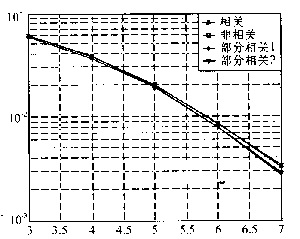
\includegraphics[height=65mm]{1.jpg}}{\hspace*{20mm}}
\end{center}
\vspace{-1.5em}
\hspace{-4em} {\xiaowu[0.75] 信噪比/dB}\\
{\centering {\xiaowu[0.75] \noindent 注:此图中的曲线对应关系与图2.1相同.}\\}
\caption{部分相干调解与相干和非相干调解平均误码性能的比较}
\label{fig:figexample1}
\end{figure}

代码如下:

\begin{lstlisting}[language=TeX]
\begin{figure}[htbp]
\begin{center}
{\rotatebox{90}{\hspace{13.5mm} \xiaowu `所有用户的平均误差比特率`}}{\hspace{15mm}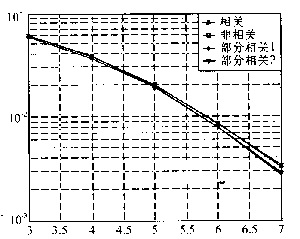
\includegraphics[height=65mm]{1.jpg}}{\hspace*{20mm}}
\end{center}
\vspace{-1.5em}
\hspace{-4em} {\xiaowu[0.75] `信噪比/dB`}\\
{\centering {\xiaowu[0.75] \noindent `注:此图中的曲线对应关系与图2.1相同.`}\\}
\caption{`部分相干调解与相干和非相干调解平均误码性能的比较`}
\label{fig:figexample1}
\end{figure}
\end{lstlisting}

主体部分是\textbackslash includegraphics[高度]\{图片\}。

另外,为了达到原图的效果,使用了\textbackslash rotatebox,旋转盒子的命令,把文字旋转90度至于图片左边。又通过用\textbackslash hspace\{\},水平间距命令及\textbackslash vspace\{\},垂直间距命令,把“信噪比/dB”放置于对齐于图片的左下角。同时使用\textbackslash centering命令把注解居中于图标题上方。以达到图2.3的效果。

字号的中括号内容表示行距设定。\LaTeX{}的行距设定在换字号大小的时候才会生效。为了使表格的注解能够比较紧凑,用0.75倍的行距比较适宜。

下\figref{figexample2}仿制《手册》22页的图3.1。

\begin{figure}[htbp]
\begin{center}
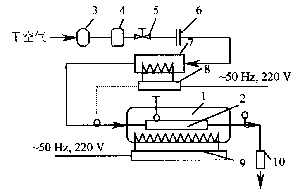
\includegraphics[height=50mm]{2.png}\\
{{\xiaowu[0.75]{1-太阳模拟器;2-单管及31个PCM容器;3-气泵;\\
4-干燥过滤器;5-手动调节阀;6-孔板流量计;\\
7-空气预热器;8,9-调功器;10-空气换热器。\\}}}
\end{center}
\caption{单管换热系统流程图}
\label{fig:figexample2}
\end{figure}

代码如下:

\begin{lstlisting}[language=TeX]
\begin{figure}[htbp]
\begin{center}
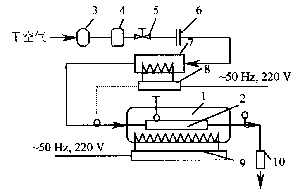
\includegraphics[height=50mm]{2.png}\\
{{\xiaowu[0.75]{`1-太阳模拟器;2-单管及31个PCM容器;3-气泵;`\\
`4-干燥过滤器;5-手动调节阀;6-孔板流量计;`\\
`7-空气预热器;8,9-调功器;10-空气换热器。`\\}}}
\end{center}
\caption{单管换热系统流程图}
\label{fig:figexample2}
\end{figure}
\end{lstlisting}

相较\figref{figexample1},\figref{figexample2}显得简单得多,我们的插图一般以这种为主。

\subsection{多个图形}
多个图形的编排与多个表格的编排基本相同,可以用小页minipage分割,或者使用subfigure子图片环境。

\figref{figexample3}展示的是《手册》23页的图2.5。

\begin{figure}[htbp]
\centering
\subfloat[分布符合1/f规律图]{%
\label{fig:subfig1}
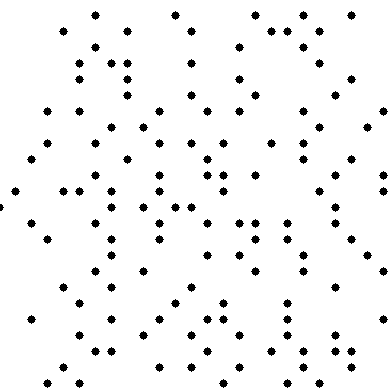
\includegraphics[height=40.8mm]{3.png}}\hspace{4em}%
\subfloat[大小与色彩符合1/f规律图]{%
\label{fig:subfig2}
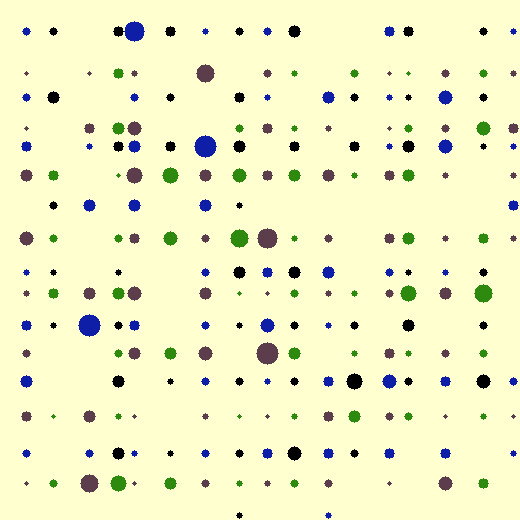
\includegraphics[height=38.4mm]{4.png}}\hspace{4em}
\subfloat[间距、大小与色彩均符合1/f规律图]{%
\label{fig:subfig3}
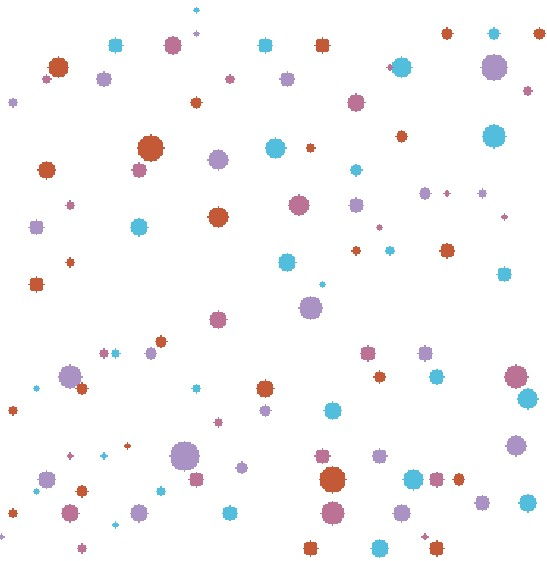
\includegraphics[height=41.7mm]{5.jpg}}
\caption{图案例}
\label{fig:figexample3}
\end{figure}

代码如下:

\begin{lstlisting}[language=TeX]
\begin{figure}[htbp]
\centering
\subfloat[`分布符合1/f规律图`]{%
\label{fig:subfig1}
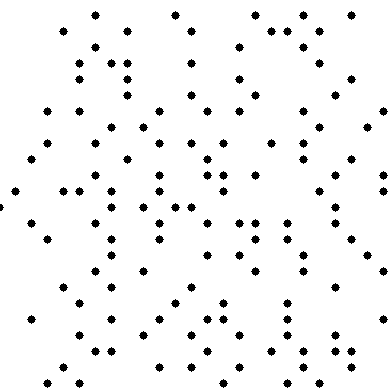
\includegraphics[height=40.8mm]{3.png}}\hspace{4em}%
\subfloat[`大小与色彩符合1/f规律图`]{%
\label{fig:subfig2}
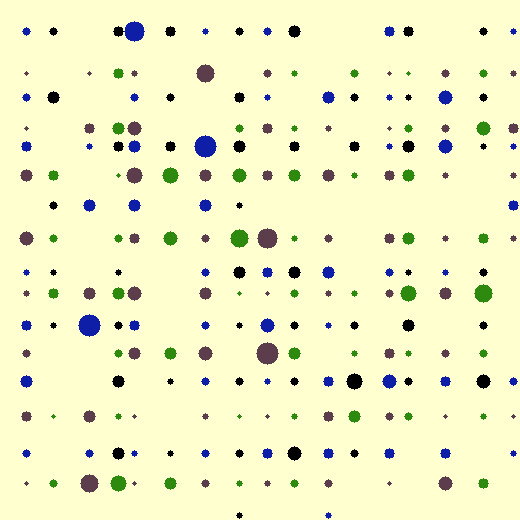
\includegraphics[height=38.4mm]{4.png}}\hspace{4em}
\subfloat[`间距、大小与色彩均符合1/f规律图`]{%
\label{fig:subfig3}
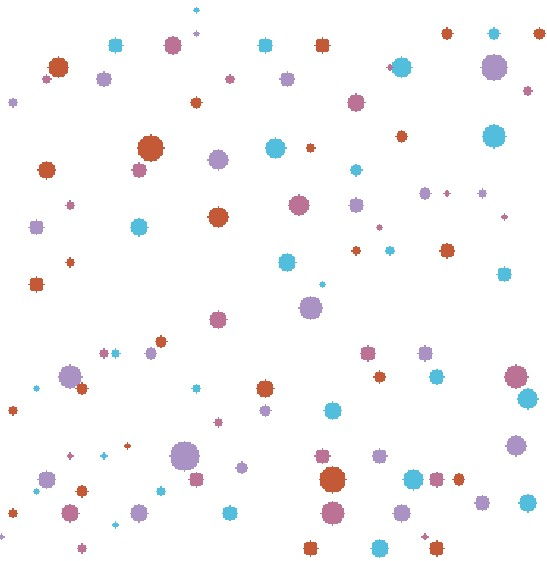
\includegraphics[height=41.7mm]{5.jpg}}
\caption{`图案例`}
\label{fig:figexample3}
\end{figure}
\end{lstlisting}

需要注意的是,图与图之间的间距,需要用水平间距命令进行调整。

\section{公式定理}
\TeX{}处理公式的能力非常强大,建议读取amsmath宏包的说明文档\textsuperscript{\cite{amsmath}}。下面举几个简单的例子,皆在公式环境equation中生成,对付不同的公式已经够了。其中的数学符号,可以在Web Equation网页中手写生成。

\begin{figure}[htbp]
\begin{center}
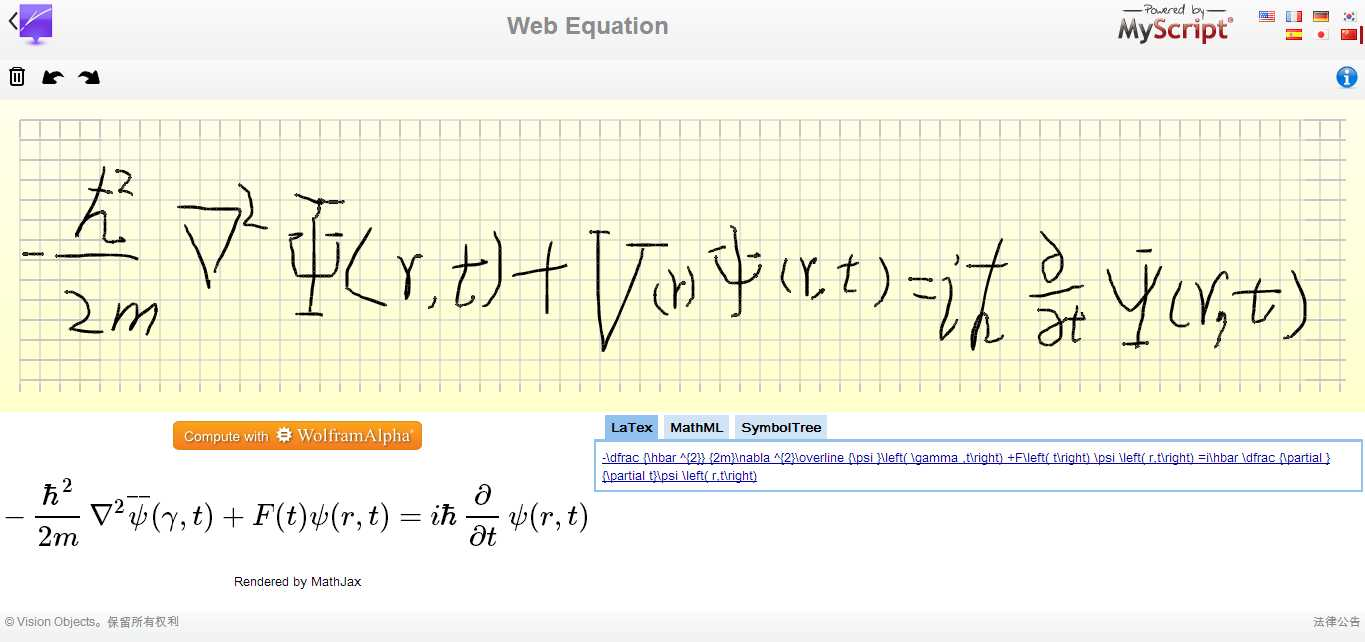
\includegraphics[width=0.9\linewidth]{wq.png}
\end{center}
\caption{用Web Equation生成\TeX{}公式代码}
\end{figure}

\subsection{单个公式}

\newcommand{\envert}[1]{\left\lvert#1\right\rvert} 
\begin{equation}\label{detK2}
\det\mathbf{K}(t=1,t_1,\dots,t_n)=\sum_{I\in\mathbf{n}}(-1)^{\envert{I}}
\prod_{i\in I}t_i\prod_{j\in I}(D_j+\lambda_jt_j)\det\mathbf{A}
^{(\lambda)}(\overline{I}|\overline{I})=0.
\end{equation} 

\begin{multline}%\tag{[b]} % 这个出现在索引中的
\int_a^b\biggl\{\int_a^b[f(x)^2g(y)^2+f(y)^2g(x)^2]
 -2f(x)g(x)f(y)g(y)\,dx\biggr\}\,dy \\
 =\int_a^b\biggl\{g(y)^2\int_a^bf^2+f(y)^2
  \int_a^b g^2-2f(y)g(y)\int_a^b fg\biggr\}\,dy
\end{multline}

\subsection{多列公式}

\begin{equation} 
\overrightarrow {p}_{i}\left( u\right) =\sum _{j=0}^{k}\overrightarrow {V}_{i}\Lambda _{i}\left( k;\overrightarrow {\beta }_{1},\ldots \overrightarrow {\beta }_{n};u\right)
\end{equation}

\begin{equation} 
\dfrac {\left| A\left( s\right) \right| ^{2}} {\left| A\left( O\right) \right| ^{2}}=\dfrac {\rho _{1}\rho _{2}} {\left( s+p_{1}\right) \left( s+\rho _{2}\right) }
\end{equation}

\section{代码高亮}
有些时候我们需要在论文中引入一段代码。
在模板中,统一使用\textbackslash listings宏包,并且设置了基本的内容格式。由于Lstlisting宏包对中文支持不太完善,可以设置中文逃逸,\textbackslash lstset\{escapeinside=``\},用键盘数字符号键“1”左边的“左引号”“`”作为逃逸标记。但请注意,在Verilog语言中,左引号为特殊符号。

C语言示例:

\begin{lstlisting}[language=C]
#include <stdio.h>
main()
{printf("Hello World!\n"); %"`你好,世界`"
}
\end{lstlisting}

\section{参考文献}
参考文献可以用thebibliography环境生成,代码如下:

\begin{lstlisting}[language=TeX]
\begin{thebibliography}{}
\bibitem[`序号`]{`引用`} `文献信息`
\bibitem[1]{b1} Wikipedia. Linux[EB/OL]. http://zh.wikipedia.org/wiki/Linux,2013-5-20/2013-5-26. 
\end{thebibliography}
\end{lstlisting}

其中[]中填入文献前标号,缺省为数字排列,\{\}中为引用标签,例如\{r1\}则可在其他地方用指令\verb|\cite{r1}|引用标签上标可以使用\textbackslash textsuperscript命令,用法与\textbackslash cite一样。

\section{致谢}
致谢可以直接使用ack环境。直接输入文字即可。

\section{附录}
使用appxchp环境,在环境里使用\textbackslash appxtoc\{标题内容\}生成符合《手册》要求的附录。同时如需要生成图或表格的标题,使用\textbackslash appxfig(图) 和\textbackslash appxtab(表) 命令。引用标题的方法与正文相同。其他的操作与正文一样。

\section{编译}
\label{sec:compile}
好的,恭喜你,你终于写完了\TeX{}原文档了。是时候开始编译了。但在这之前,你还需要以下步骤:

1、创建一个空文件夹,名称如:gdutthesis

2、把thesis.tex、gdutthesis.cls、mygdut.sty、makepdf.bat、makefile三个文件放到你新建的文件夹里。

3、在这个新文件夹下建立两个新的空文件夹,data和figure。

4、把除thesis.tex以外的\TeX{}源文件放到Data下。记得在thesis.tex里用\textbackslash input命令加载它们。

5、把一切需要调用的图片都放在figure文件夹下面。

6、这个时候,可以开始编译了。

7、在命令行中,用cd命令定位到到你的\TeX{}源文件目录下,输入以下的代码,即可以编译thesis.tex文件了。\TeX{}文件需要经过三次编译才能正确显示效果\textsuperscript{\cite{shouce}}。 

\begin{lstlisting}[language=TeX]
xelatex thesis
xelatex thesis
xelatex thesis
\end{lstlisting}

8、最后祈祷一下吧,理论上不出错的话你就能得到一份比较不错的论文了。

9、补充一点,假如你觉得以上的步骤相当复杂,那么你可以直接在这份PDF文件的源文件夹下面操作。

\input{data/chap04}

% 参考文献
\begin{thebibliography}{20}
\bibitem{Linux} Wikipedia. Linux[EB/OL]. http://zh.wikipedia.org/wiki/Linux,2013-5-20/2013-5-26. 
\bibitem{Bai.linux} Baidu. Linux[EB/OL]. http://baike.baidu.com/view/1634.html,2013-05-22/2013-5-26.
\bibitem{CTEX} C\TeX{}. \TeX{}[EB/OL]. http://www.ctex.org/TeX/,2005-01-06/2013-5-26. 
\bibitem{WYSIWYG} Wikipedia. WYSIWYG[EB/OL].\\
http://en.wikipedia.org/wiki/WYSIWYG,2013-05-30/2013-5-30.
\bibitem{rumen} 陈志杰,赵书钦,李树钧,万福永. \LaTeX{}入门与提高(第二版)[M]. 北京:高等 教育出版社,2006.
\bibitem{ubuntu} Wikipedia. Ubuntu[EB/OL]. http://zh.wikipedia.org/wiki/Ubuntu,2013-5-13/2013-5-26.
\bibitem{b6} Karl Berry. \TeX{} Live 指南[EB/OL].\\
http://www.tug.org/texlive/doc/texlive-zh-cn/texlive-zh-cn.pdf,2012-6/2013-5.
\bibitem{TeXMaker} Wikipedia. \TeX{}Maker[EB/OL]. http://en.wikipedia.org/wiki/Texmaker,2013-5-9/2013-5-26.
\bibitem{xeCJK} 孙文昌. xeCJK宏包指南[EB/OL].\\
http://wenku.baidu.com/view/0b3e53abdd3383c4bb4cd267.html,2012-01-13/2013-5-26.
\bibitem{zhongwen} lins05. 真正的Linux下的中文\LaTeX{}解决方案: CTeX + xeCJK + XeTEX[EB/OL]. \\http://www.360doc.com/content/11/1112/15/532901\_163797486.shtml,2011-8-6/2013-5-26.
\bibitem{point} Wikipedia. Point(typography)[EB/OL]. \\
https://en.wikipedia.org/wiki/Point\_(typography),2013-3-12/2013-5-26.
\bibitem{2e} 胡伟. \LaTeX{} 2ε完全学习手册[M]. 北京:清华大学出版社,2011. 
\bibitem{graphics} Keith Reckdahl. Using Import graphics in \LaTeX{} 2ε[EB/OL].\\
http://www.ctex.org/documents/latex/graphics/,1997-11-15/2013-5-26.
\bibitem{amsmath} American Mathematical Society. User's Guide for the amsmath Package[EB/OL].\\
ftp://ftp.ams.org/pub/tex/doc/amsmath/amsldoc.pdf,2002-2-25/2013-5-26.
\bibitem{shouce} 罗振东,葛向阳. 排版软件\LaTeX{}简明手册(第二版)[M]. 北京: 电子工业出版社,2004.
\end{thebibliography}


% 致谢
\begin{ack}
同时感谢华南师范大学的潘伟洲同学以及清华大学、国防科技大学、上海交通大学等学校\LaTeX{}论文模板开发人员。因为他们之前的努力,致使我在短时间内能够掌握\TeX{}排版,及模板运作方式。
\end{ack}


% 附录
\backmatter
\begin{appxchp}
\appxtle{附录样式示例}
这是《手册》27页的附录A示例。

引用示例:如图~\ref{appxfig:appxexampleA}

\begin{figure}[htbp]
\begin{center}
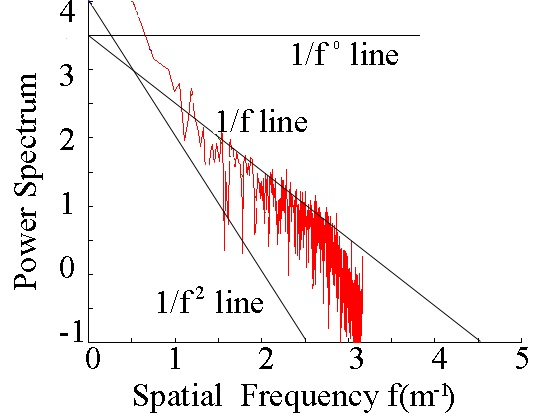
\includegraphics[width=0.9\linewidth]{fulu1.jpg}
\end{center}
\appxfig{频谱图}
\label{appxfig:appxexampleA}
\end{figure}

\end{appxchp}

\begin{appxchp}
\appxtle{图片、表格、公式示例}
这是前面内容的复制粘贴,目的在于附录样式的展示

\begin{figure}[htbp]
\centering
\subfloat[分布符合1/f规律图]{%
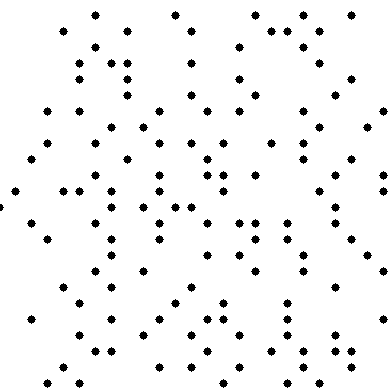
\includegraphics[height=40.8mm]{3.png}}\hspace{4em}%
\subfloat[大小与色彩符合1/f规律图]{%
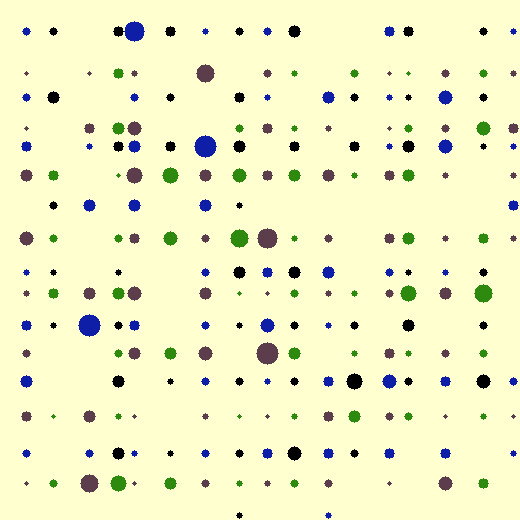
\includegraphics[height=38.4mm]{4.png}}\hspace{4em}
\subfloat[间距、大小与色彩均符合1/f规律图]{%
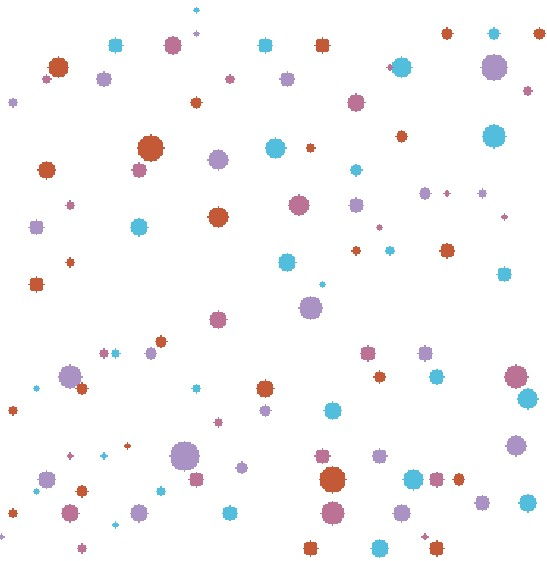
\includegraphics[height=41.7mm]{5.jpg}}
\appxfig{图案例}
\end{figure}

\begin{table}[htbp]
\appxtab{并排子表格}
\begin{center}
\subfloat[第一个子表格]{
\begin{tabularx}{0.3\linewidth}{Z|Z}\toprule
111 & 222 \\\midrule
222 & 333 \\\bottomrule
\end{tabularx}}\hspace{0.15\linewidth}
\subfloat[第二个子表格]{
\begin{tabularx}{0.3\linewidth}{Z|Z}\toprule
111 & 222 \\\midrule
222 & 333 \\\bottomrule
\end{tabularx}}
\end{center}
\end{table}

附录中的公式不需要加编号,所以记得使用无编号的公式环境。

\begin{equation*} 
\left(\begin{array}{c|c} 
1 & 2 \\ 
\hline 3 & 4 \end{array}\right) 
\end{equation*}   

\begin{eqnarray*}
f(x) & = & \cos x \\ 
f'(x) & = & -\sin x \\ 
\int_{0}^{x} f(y)\,dy & = & \sin x 
\end{eqnarray*} 

\begin{eqnarray*} 
\sin x & = & x -\frac{x^{3}}{3!} +\frac{x^{5}}{5!}-{} \nonumber\\ 
	& & {}-\frac{x^{7}}{7!}+{}\cdots 
\end{eqnarray*}

\end{appxchp}
%\input{data/appendix02}

\end{document}
%%
